\chapter{PERSYARATAN SISTEM }

\label{chapter:PERSYARATAN SISTEM}

\section{Deskripsi Pengguna}
Target pengguna utama dari aplikasi Food AI Rescue (FAR) secara umum adalah seluruh entitas yang terlibat dalam ekosistem pengelolaan surplus makanan, rantai pasok logistik sosial, dan penerima manfaat di tingkat komunitas. Sistem ini memfasilitasi kolaborasi multi-pihak yang dirancang agar ramah pengguna (user-friendly), baik bagi masyarakat awam, pelaku usaha, maupun tim manajerial. Untuk memetakan kebutuhan sistem, pengguna aplikasi ini didetailkan ke dalam segmentasi dan peran (role) sebagai berikut:

% \subsection{Segmentasi Pengguna}

\begin{figure}[htbp]
    \centering
    \includegraphics[width=1\textwidth]{image/bab2/segmentasi.png}
    \caption{Segmentasi Pengguna Food AI Rescue}
    \label{fig:segmentasi}
\end{figure}

\begin{enumerate}
    \item \textbf{Donatur Individu}
    \begin{itemize}
        \item \textbf{Segmen/Profil}: Masyarakat perorangan atau pelaku usaha skala mikro yang memiliki kelebihan produksi makanan dalam jumlah kecil (skala rumah tangga).
        \item \textbf{Peranan dan Hak Akses Utama}: Memiliki hak untuk mengunggah data makanan surplus, memperbarui status ketersediaan (\textit{inventory}), serta melakukan serah terima secara langsung. Pada saat serah terima menggunakan fitur Janji Temu (COD), pengguna wajib memindai QR Code milik Penerima sebagai bukti distribusi yang sah. Selain itu, donatur memiliki akses untuk memantau Dasbor Dampak Sosial (SROI) yang memuat laporan total porsi terselamatkan dan estimasi pengurangan emisi jejak karbon (CO$_2$).
        \item \textbf{Hak Akses AI}: Memiliki akses ke fitur bawaan AI \textit{Quality Verification}. Sebelum donasi dipublikasikan, donatur wajib memindai foto makanan menggunakan kamera AI ini guna memastikan kelayakan fisik dan higienitas visual. Selain itu, donatur juga dapat memindai (\textit{scan}) bahan makanan untuk mendapatkan rekomendasi resep masakan dari sistem.
    \end{itemize}
    \item \textbf{Donatur Kelompok/Korporat (Mitra Penyedia)}
    \begin{itemize}
        \item \textbf{Segmen/Profil}: Pelaku bisnis skala besar di sektor \textit{Hospitality, Restaurant, and Cafe} (HORECA) seperti restoran, hotel, atau usaha katering berskala komersial.
        \item \textbf{Peranan dan Hak Akses Utama}: Memiliki peranan dan hak akses operasional yang sama persis dengan Donatur Individu, mulai dari siklus manajemen distribusi (unggah surplus, update \textit{inventory}, pindai QR serah terima) hingga pemantauan laporan di Dasbor Dampak Sosial (SROI).
        \item \textbf{Hak Akses Khusus (Spesial) AI}: Sebagai nilai tambah (\textit{value}) untuk mendukung kampanye pemasaran dan \textit{Corporate Social Responsibility} (CSR) perusahaan, donatur tingkat kelompok/korporat dibekali hak istimewa terhadap dua modul AI generatif eksklusif, yaitu:
        \begin{itemize}
            \item \textbf{\textit{Generate Image} Kemasan}: Hak spesial untuk menghasilkan gambar desain prototipe bungkus atau kemasan makanan.
            \item \textbf{\textit{Generate} Konten Media Sosial}: Hak spesial untuk secara otomatis menghasilkan gambar visual desain (lengkap dengan stiker verifikasi AI dan logo perusahaan) sekaligus memproduksi konten tulisan (\textit{copywriting}) promosi yang siap diunggah ke platform media sosial.
        \end{itemize}
    \end{itemize}
    \item \textbf{Penerima (Mitra Penerima)}
    \begin{itemize}
        \item \textbf{Segmen/Profil}: Masyarakat di kawasan rentan pangan, panti asuhan, dewan kemakmuran masjid (DKM), atau warga prasejahtera di desa sasaran yang membutuhkan bantuan makanan.
        \item \textbf{Peranan dan Hak Akses}: Memiliki akses untuk mencari menu makanan terdekat, melakukan proses klaim (booking) guna mengunci stok dan mencegah insiden pengambilan ganda (double-claim) oleh pihak lain, memilih metode pengambilan, dan menyajikan QR Code miliknya untuk dipindai saat makanan tiba.
        \item \textbf{Hak Akses Khusus AI}: Penerima diberikan akses ke fitur AI \textit{Quality Verification} untuk memindai kelayakan fisik dan higienitas visual makanan sebelum dikonsumsi, fitur Forum Request untuk memublikasikan kebutuhan pangan spesifik, serta memberikan ulasan (\textit{feedback}).
    \end{itemize}
    \item \textbf{Relawan}
    \begin{itemize}
        \item \textbf{Segmen/Profil}: Pemuda lokal, warga desa, atau masyarakat umum yang bertindak secara sukarela (\textit{crowdsourcing}) sebagai armada logistik sosial.
        \item \textbf{Peranan dan Hak Akses}: Mengakses daftar misi pengantaran, melakukan penjemputan makanan dari lokasi Donatur, dan mengantarkannya secara langsung ke titik lokasi Penerima. Relawan memegang otoritas validasi lapangan dengan hak akses wajib pindai (\textit{mandatory scan}) QR Code milik Penerima sebagai syarat mutlak penyelesaian transaksi distribusi.
    \end{itemize}
    \item \textbf{Admin Pengelola}
    \begin{itemize}
        \item \textbf{Segmen/Profil}: Tim manajerial dan pengawas operasional harian yang bertugas mengelola sistem secara administratif di tingkat komunitas.
        \item \textbf{Peranan dan Hak Akses}: Memiliki hak akses dashboard admin untuk memverifikasi keabsahan pendaftaran akun baru secara manual, membekukan atau memblokir akun yang terbukti melakukan penyalahgunaan, menindaklanjuti laporan negatif, serta memantau Dasbor Statistik makro yang menampilkan peta panas (\textit{heatmap}) sebaran wilayah donasi dan kalkulasi SROI keseluruhan.
    \end{itemize}
    \item \textbf{Super Admin}
    \begin{itemize}
        \item \textbf{Segmen/Profil}: Pengembang sistem (Tim IT / Programmer).
        \item \textbf{Peranan dan Hak Akses}: Memiliki tingkat hak akses paling tinggi dan menyeluruh pada sisi \textit{backend} aplikasi. Super Admin bertugas untuk melakukan pemeliharaan server secara berkala (\textit{maintenance}), menangani perbaikan apabila terdapat laporan \textit{bug} dari sistem, dan menjaga stabilitas basis data secara penuh.
    \end{itemize}
\end{enumerate}

\newpage

\section{Gambaran Sistem Saat Ini}
Gambaran sistem yang berjalan saat ini (As-Is) pada ekosistem penyaluran donasi surplus makanan di masyarakat masih sepenuhnya mengandalkan metode konvensional secara manual dan tidak terstruktur. Hingga saat ini, belum ada satu pun aplikasi khusus atau sistem terintegrasi yang memfasilitasi tata kelola operasional logistik donasi pangan secara digital yang disertai dengan jaminan standar keamanan mutu. Startup JagoAI sebagai pihak inovator juga belum memiliki platform pusat kendali (command center) untuk memonitor aktivitas donasi, memvalidasi kelayakan makanan secara otomatis, serta melacak pergerakan relawan kurir secara terpusat.
% \\
% Berdasarkan hasil observasi di lapangan, seluruh pencatatan data ketersediaan surplus makanan dan riwayat penyalurannya masih tidak terdokumentasi dengan baik atau hanya dicatat secara manual. Selain itu, proses pengecekan kelayakan dan keamanan pangan hanya mengandalkan observasi visual dengan mata telanjang oleh pihak donatur tanpa standar higienitas yang baku. Satu-satunya perangkat lunak yang umum digunakan dalam ekosistem penyaluran donasi saat ini hanyalah aplikasi pesan instan pihak ketiga (seperti grup WhatsApp), yang sekadar dimanfaatkan sebagai sarana komunikasi dasar, bukan sebagai sistem manajemen logistik terpadu maupun penyimpan basis data (database). Ketiadaan sistem yang terintegrasi ini menyebabkan rantai informasi penjemputan sering terputus, tingginya risiko ancaman kesehatan bagi penerima akibat kelalaian manusia (human error) dalam memvalidasi makanan, serta lambatnya proses distribusi yang berujung pada membusuknya makanan sebelum disalurkan sehingga tetap berakhir menjadi tumpukan limbah makanan (food waste).
\subsection{Analisis Proses Bisnis}
Pada sistem manual, proses berbagi makanan berlebih berjalan secara sporadis, linear, dan tidak terstruktur. Ketika rumah tangga, penyelenggara acara, atau pelaku industri (seperti restoran dan hotel) memiliki surplus makanan, mereka harus mencari sendiri fasilitas sosial atau individu yang membutuhkan secara tatap muka atau melalui pesan singkat yang terbatas. Ketiadaan rantai pasok logistik yang terpusat ini menyebabkan waktu terbuang percuma hanya untuk mencari siapa yang bersedia menerima makanan tersebut. Akibatnya, banyak makanan yang awalnya masih layak konsumsi menjadi basi atau kedaluwarsa di tengah jalan, sehingga pada akhirnya tetap berujung dibuang ke Tempat Pembuangan Akhir (TPA) dan memicu masalah emisi gas rumah kaca.

\begin{figure}[htbp]
    \centering
    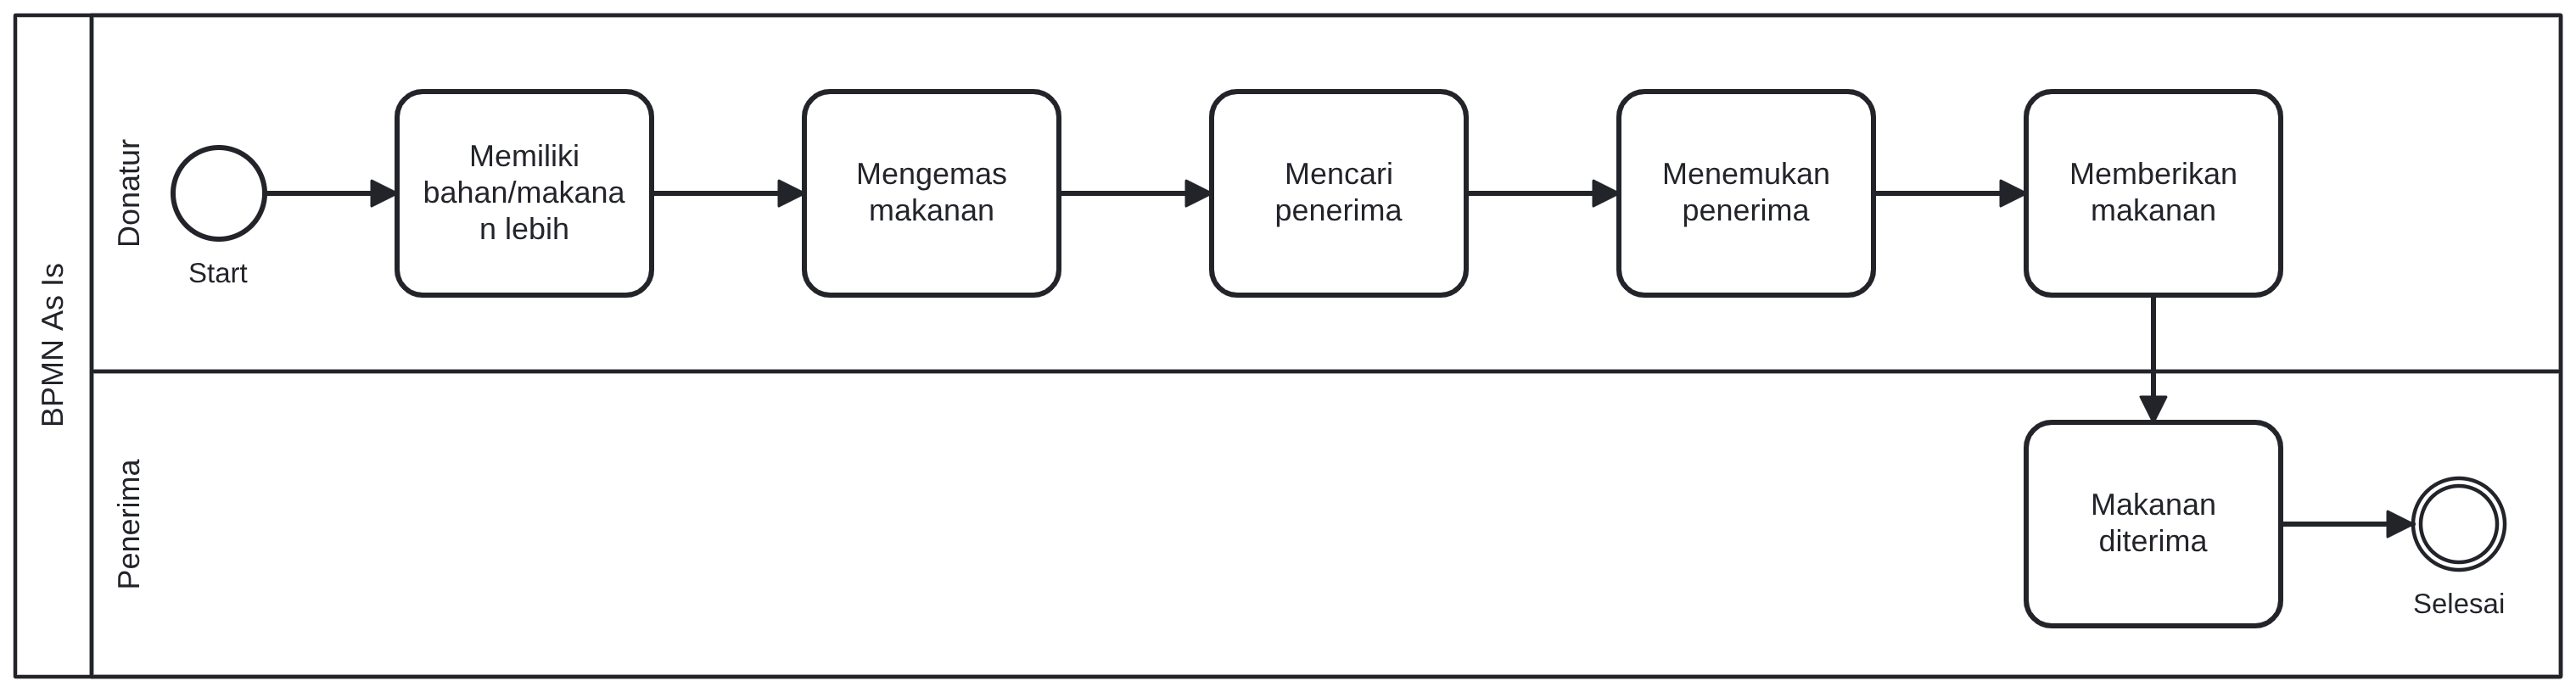
\includegraphics[width=1\textwidth]{image/bpmnAsIs.png}
    \caption{Proses Bisnis Sistem Saat Ini (BPMN As-Is)}
    \label{fig:bpmnAsIs}
\end{figure}
\begin{figure}[htbp]
    \centering
    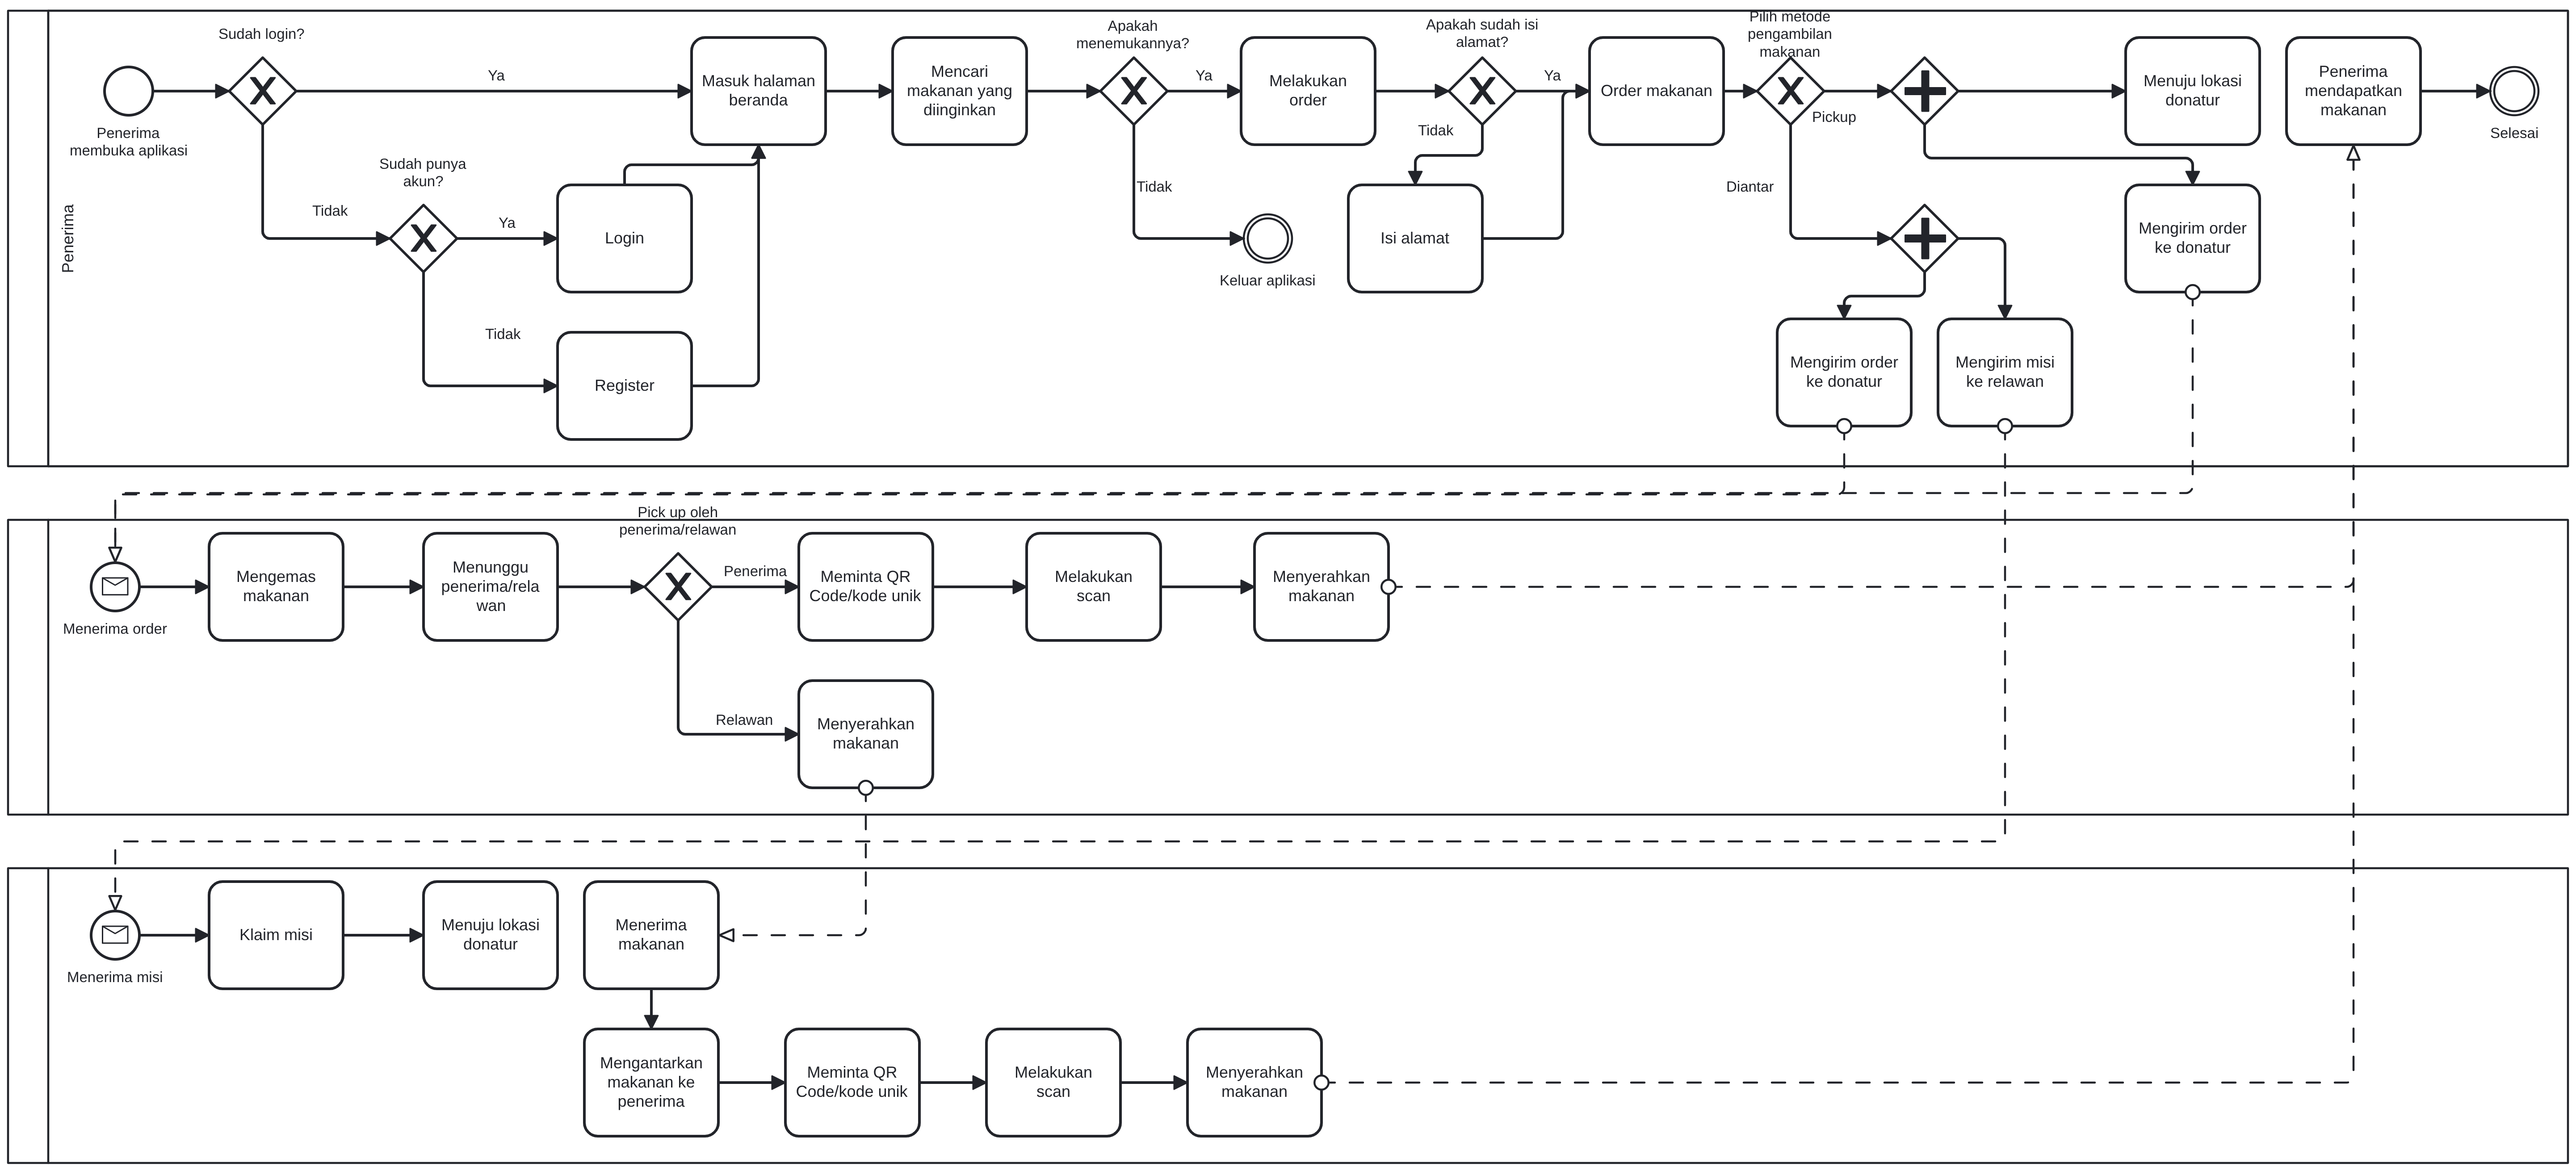
\includegraphics[width=1\textwidth]{image/bpmnToBe.png}
    \caption{Proses Bisnis Sistem Usulan (BPMN To-Be)}
    \label{fig:bpmnToBe}
\end{figure}

\newpage

\subsection{Pengalaman Pengguna}
Guna memastikan bahwa platform FoodAI Rescue yang dikembangkan dapat menyelesaikan permasalahan secara akurat dan tepat sasaran, penelitian ini menerapkan pendekatan desain berpusat pada manusia (Human-Centered Design). Pendekatan ini secara spesifik memetakan pengalaman dari target pengguna utama di lapangan—yakni pihak donatur, penerima donasi, dan relawan logistik—ketika mereka masih melakukan proses penyaluran surplus makanan secara manual atau konvensional (As-Is). Hasil pemetaan permasalahan tersebut kemudian dituangkan ke dalam tiga artefak User Experience (UX), meliputi User Persona, Empathy Map, dan User Journey Map, yang dijabarkan sebagai berikut:

\begin{figure}[htbp]
    \centering
    \includegraphics[width=1\textwidth]{image/bab2/user_persona_individu_donor.png}
    \caption{User Persona Individu Donor}
    \label{fig:userPersonaIndividuDonor}
\end{figure}
\begin{figure}[htbp]
    \centering
    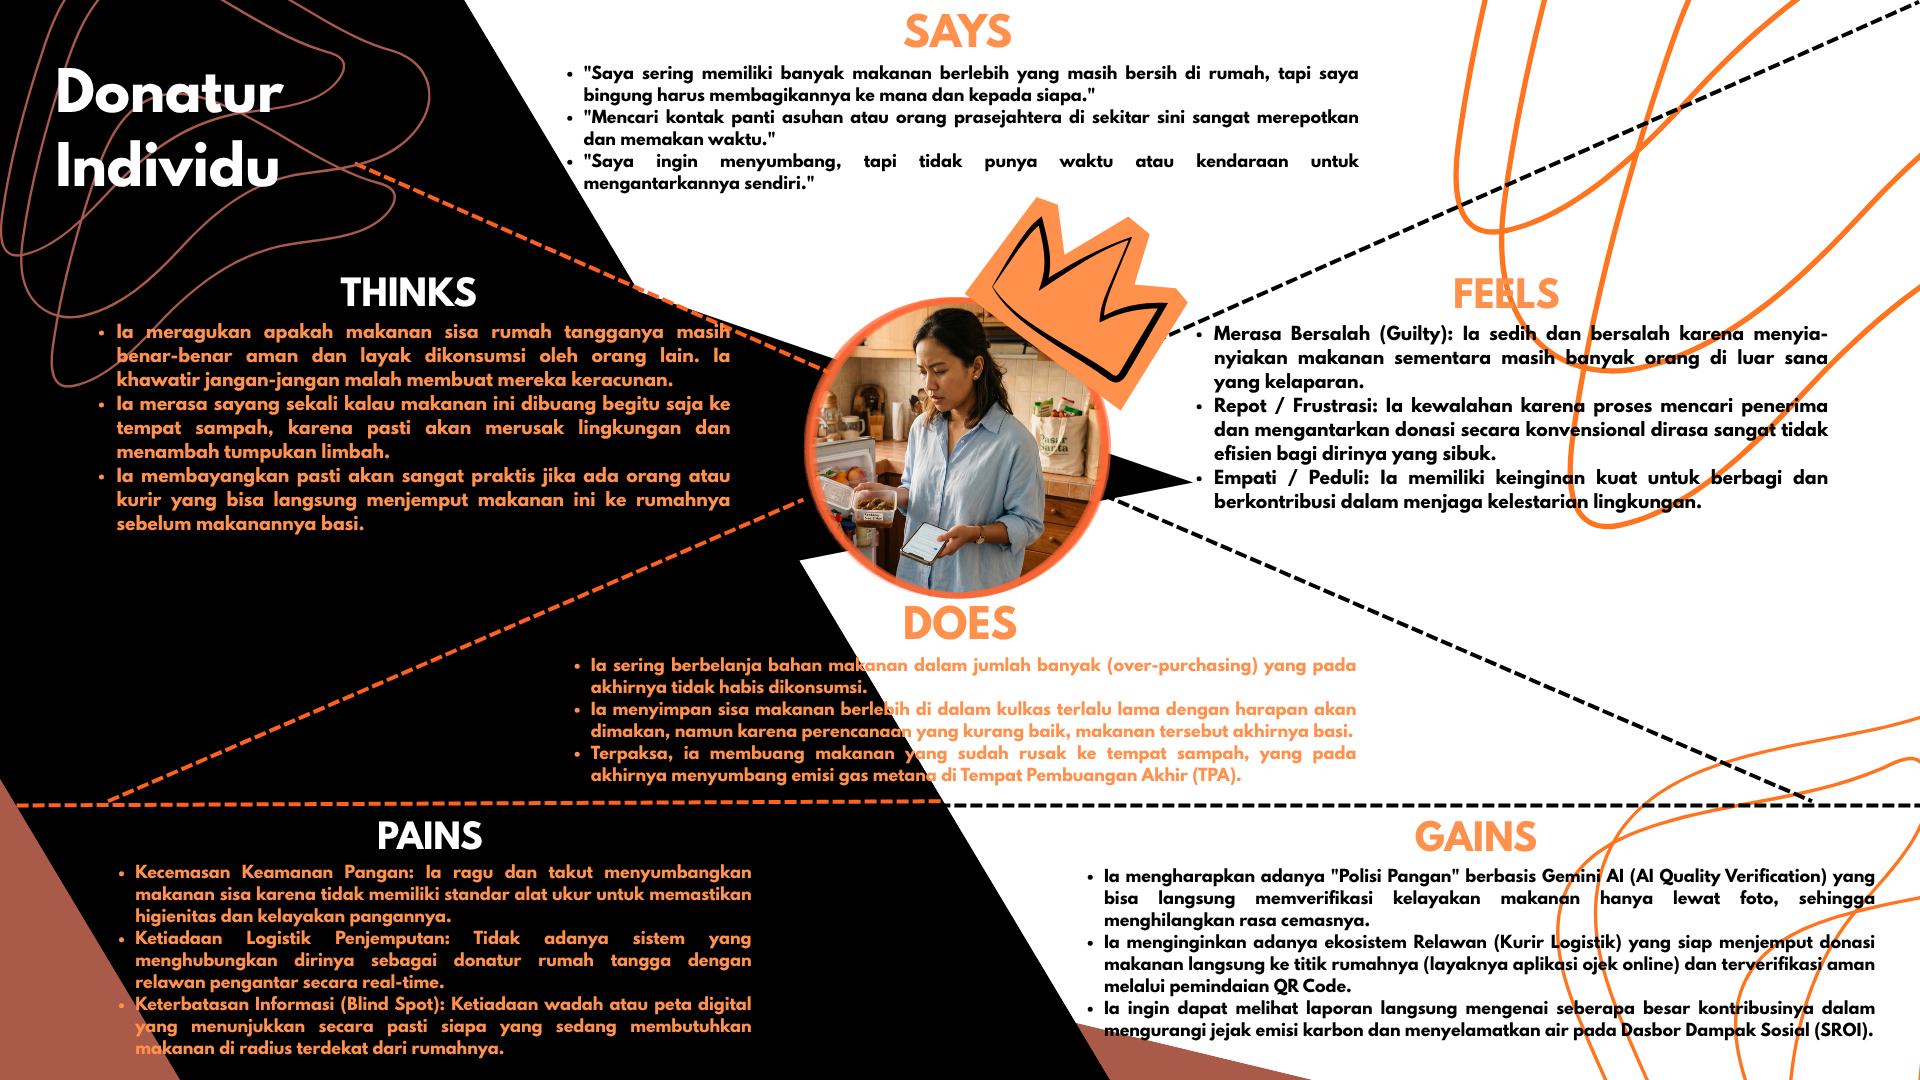
\includegraphics[width=1\textwidth]{image/bab2/segmentasi/empati_map/thinks_and_feels/donatur_individu.png}
    \caption{Empati Map Individu Donor}
    \label{fig:empatiMapIndividuDonor}
\end{figure}

\begin{figure}[htbp]
    \centering
    \includegraphics[width=1\textwidth]{image/bab2/user_persona_korporat_donor.png}
    \caption{User Persona Korporat Donor}
    \label{fig:userPersonaKorporatDonor}
\end{figure}
\begin{figure}[htbp]
    \centering
    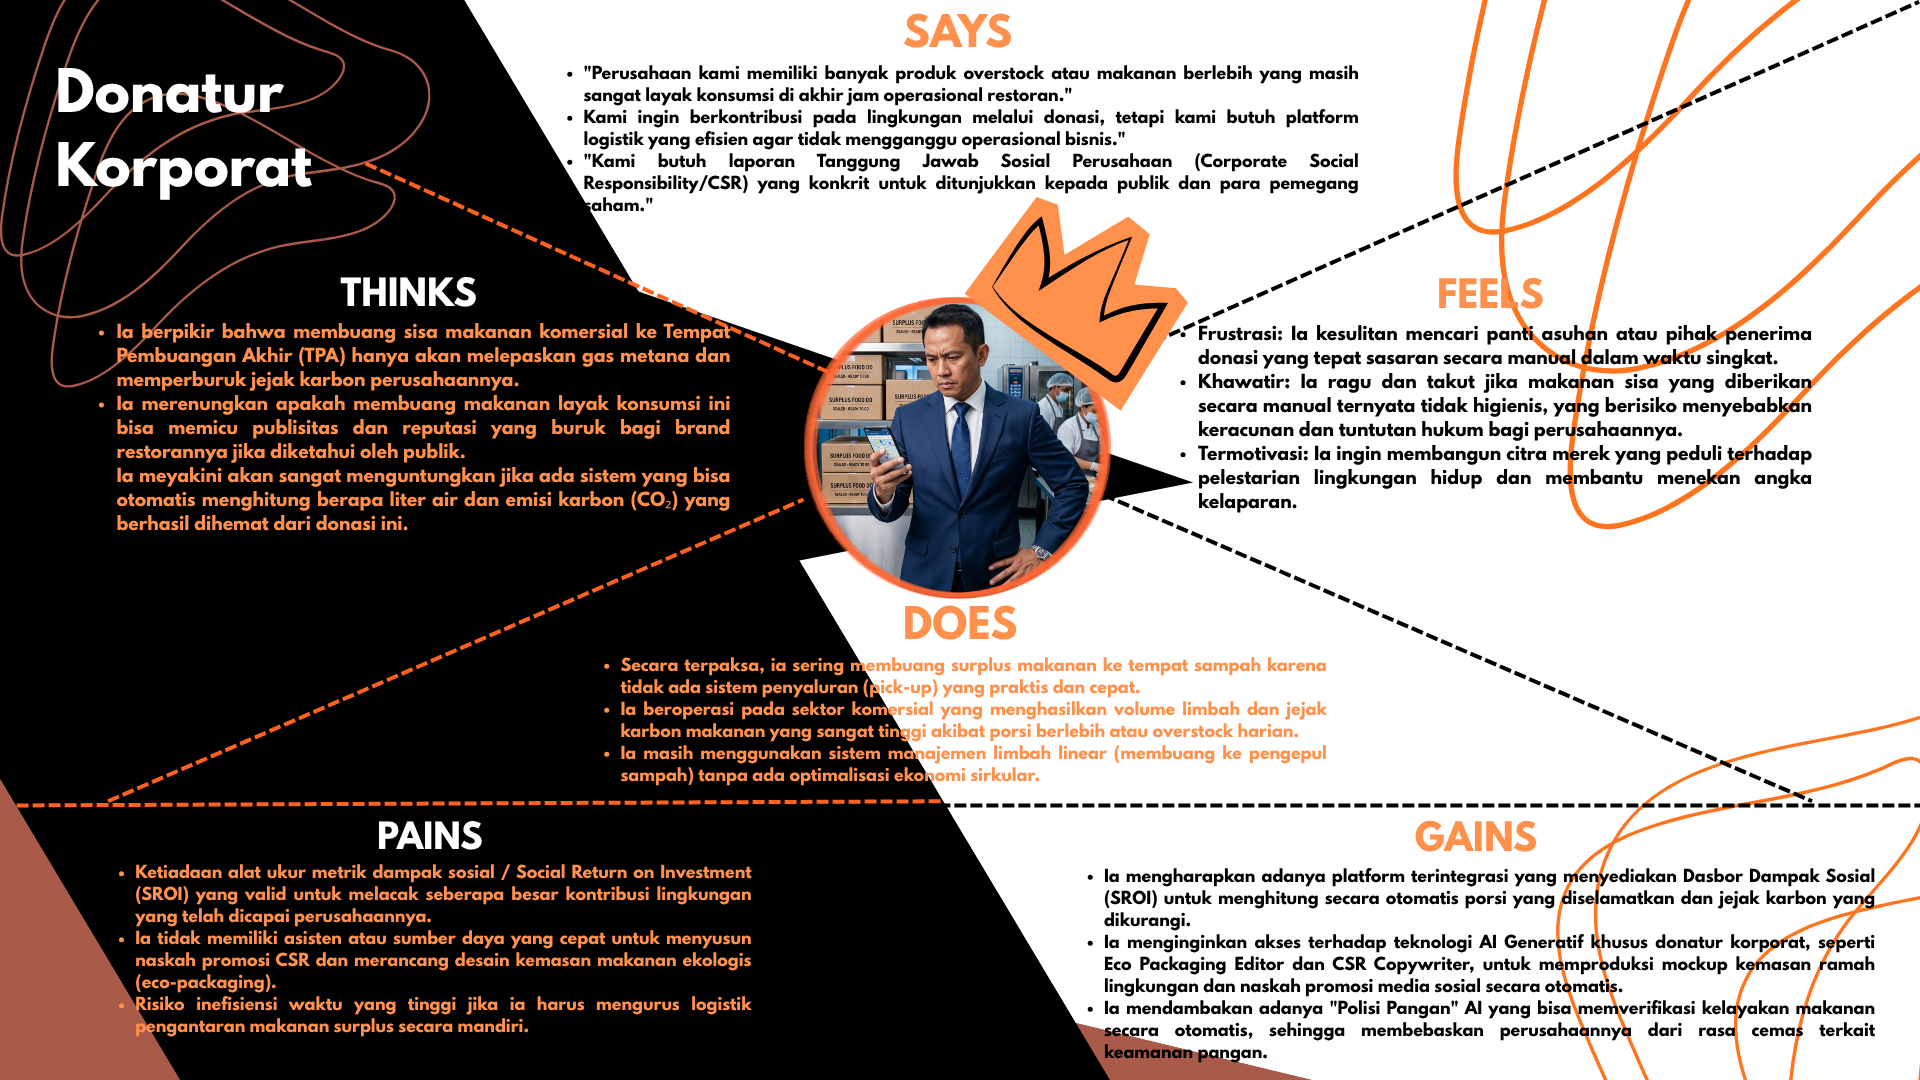
\includegraphics[width=1\textwidth]{image/bab2/segmentasi/empati_map/thinks_and_feels/donatur_korporat.png}
    \caption{Empati Map Korporat Donor}
    \label{fig:empatiMapKorporatDonor}
\end{figure}

\begin{figure}[htbp]
    \centering
    \includegraphics[width=1\textwidth]{image/bab2/user_persona_penerima.png}
    \caption{User Persona Penerima}
    \label{fig:userPersonaPenerima}
\end{figure}
\begin{figure}[htbp]
    \centering
    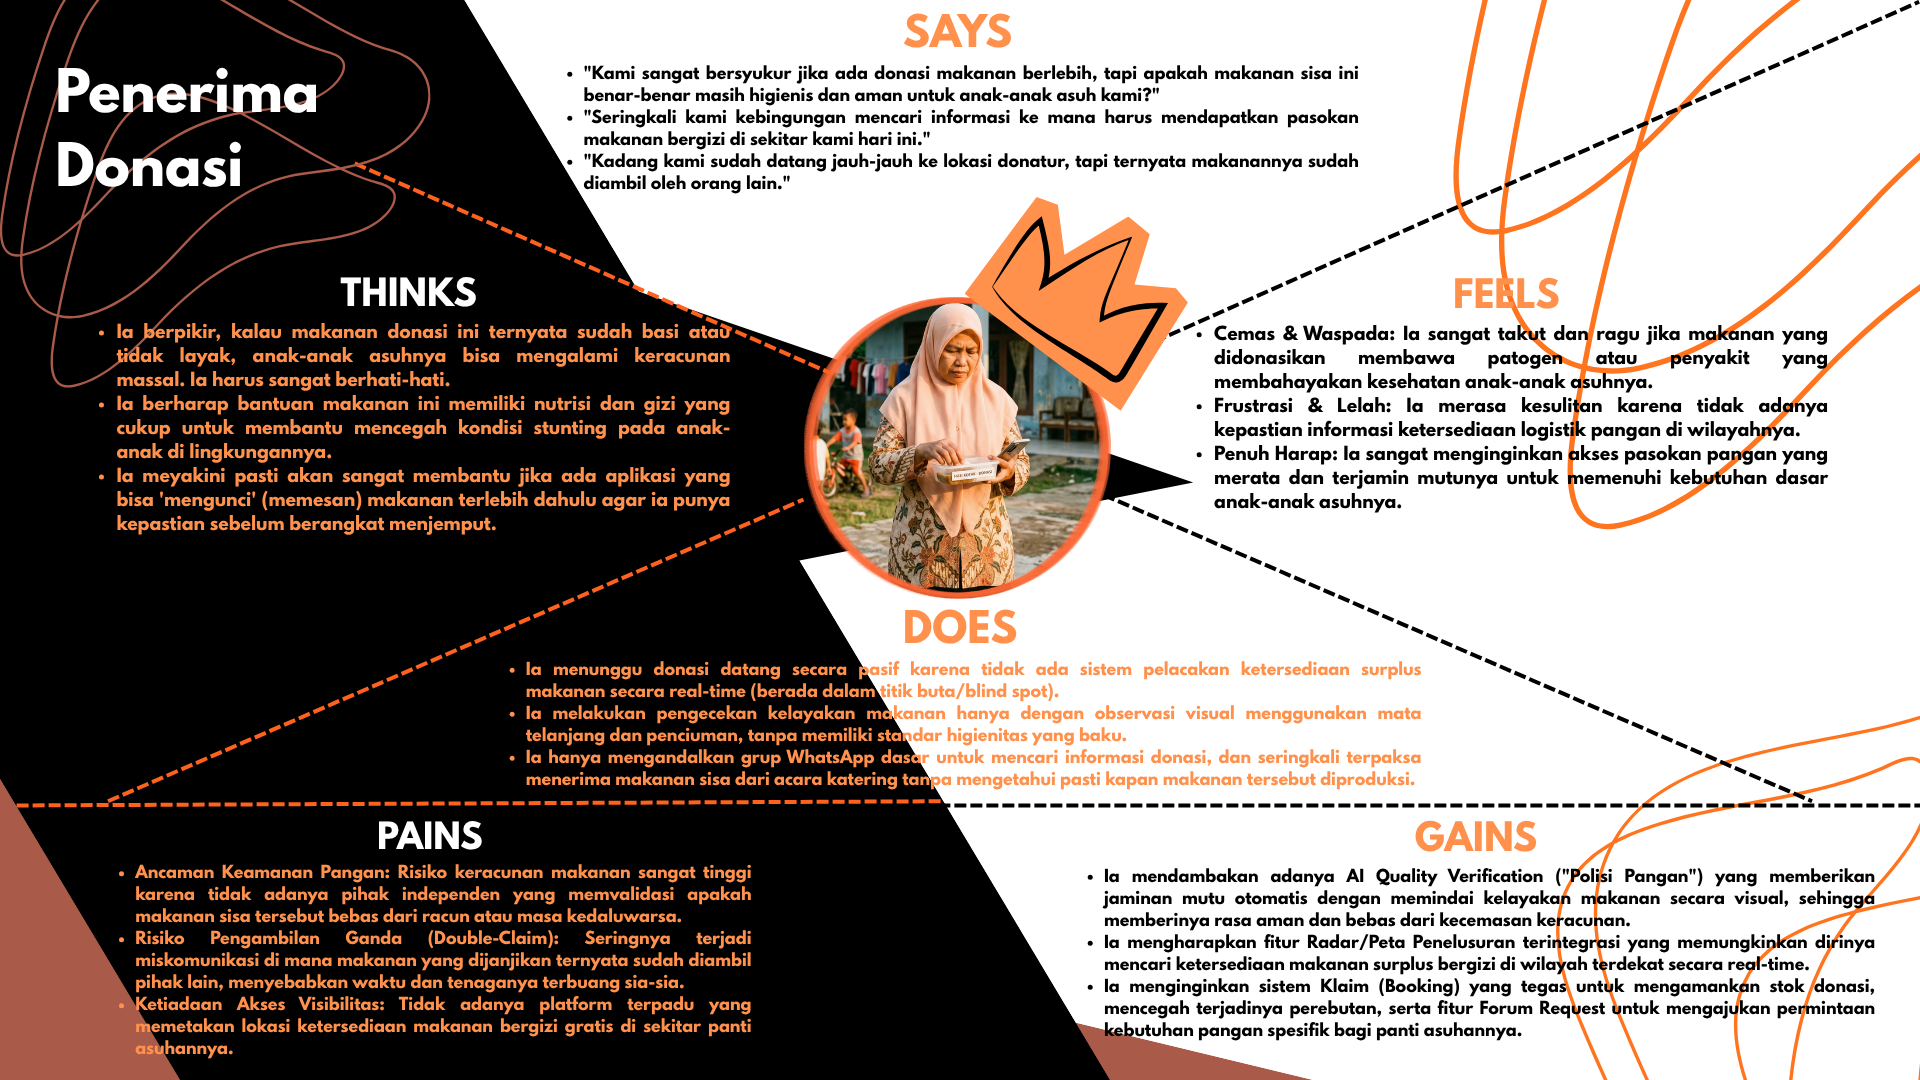
\includegraphics[width=1\textwidth]{image/bab2/segmentasi/empati_map/thinks_and_feels/penerima.png}
    \caption{Empati Map Penerima}
    \label{fig:empatiMapPenerima}
\end{figure}

\begin{figure}[htbp]
    \centering
    \includegraphics[width=1\textwidth]{image/bab2/user_persona_relawan.png}
    \caption{User Persona Relawan}
    \label{fig:userPersonaRelawan}
\end{figure}
\begin{figure}[htbp]
    \centering
    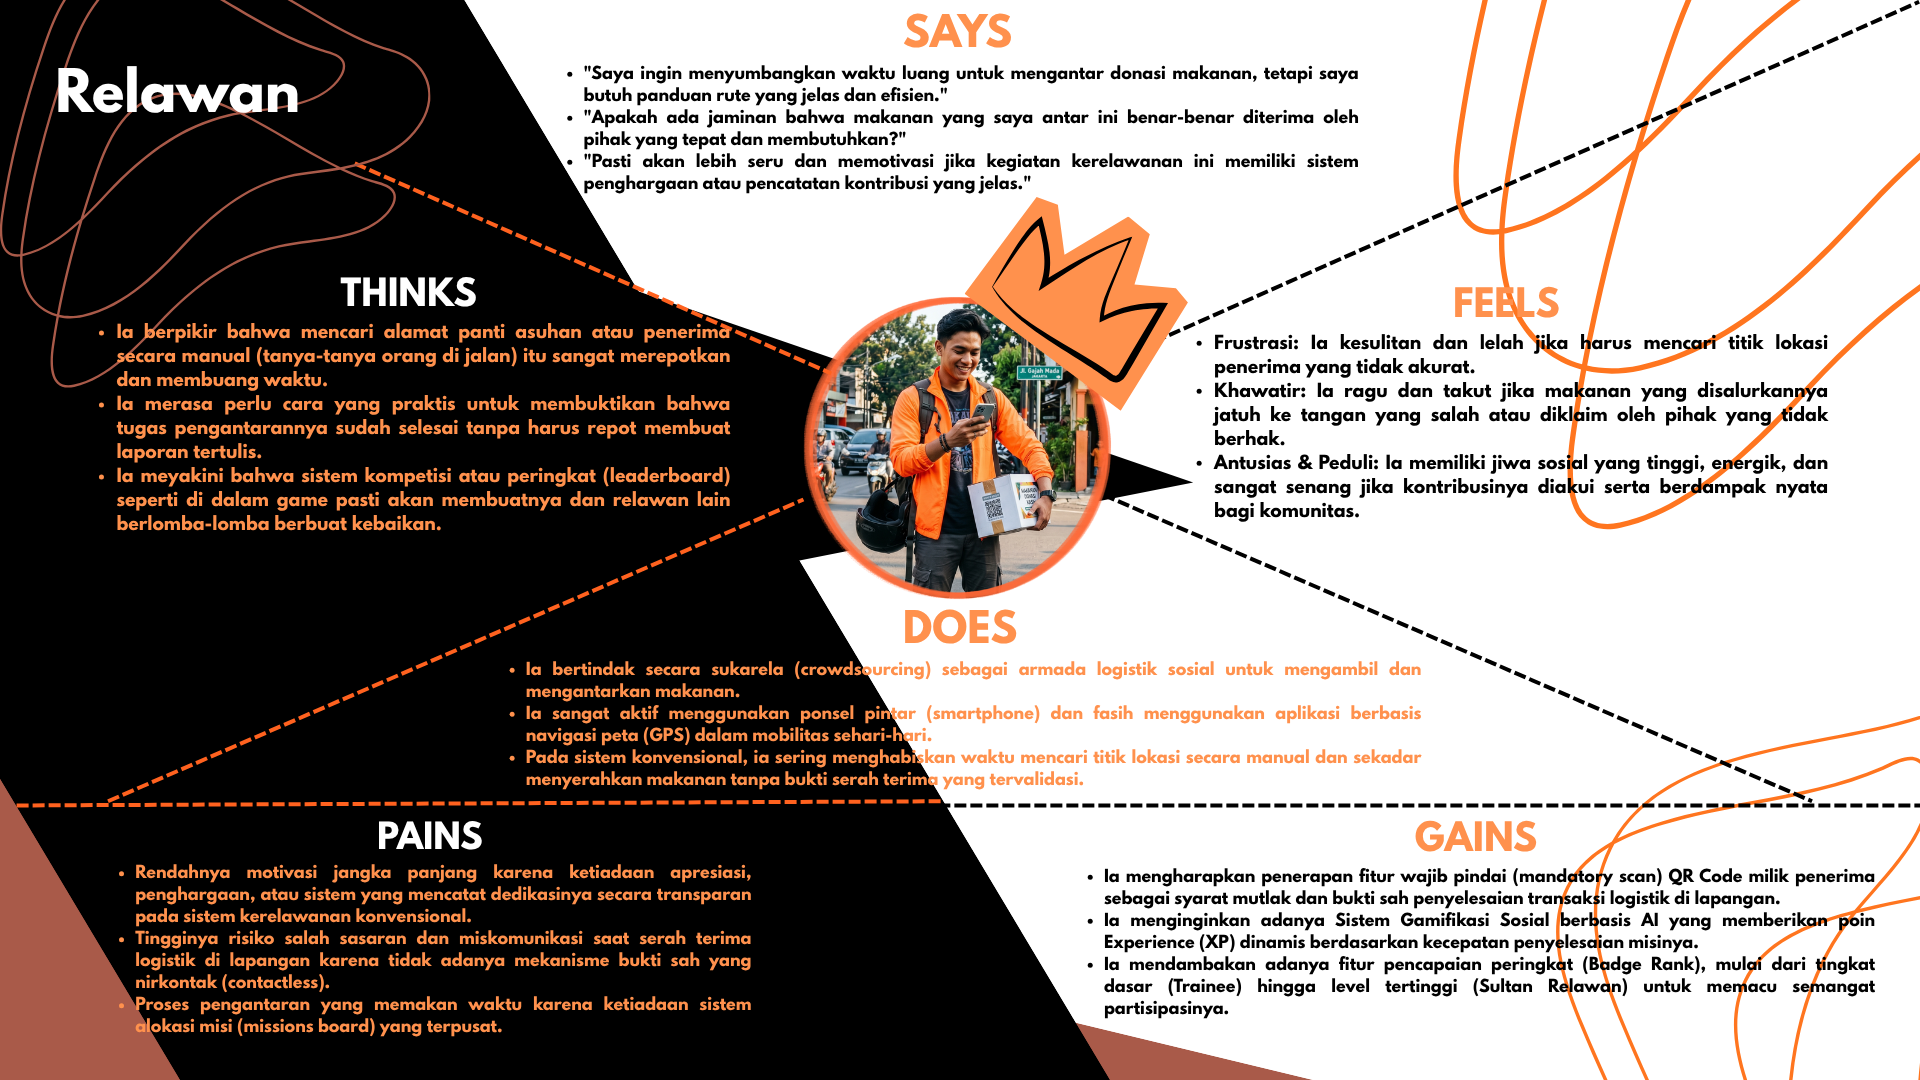
\includegraphics[width=1\textwidth]{image/bab2/segmentasi/empati_map/thinks_and_feels/relawan.png}
    \caption{Empati Map Relawan}
    \label{fig:empatiMapRelawan}
\end{figure}
\clearpage

\section{Identifikasi Aplikasi Sejenis}
Tahapan identifikasi aplikasi sejenis dilakukan guna memetakan berbagai produk atau layanan perangkat lunak di pasar (existing solutions) yang memiliki kemiripan fungsionalitas dengan sistem yang sedang diusulkan. Observasi ini ditujukan untuk menganalisis celah kelemahan (gap) dari platform pendahulu, sehingga rancangan aplikasi FoodAI Rescue mampu menghadirkan nilai tambah (value proposition) yang lebih kuat dan relevan bagi target penggunanya—seperti donatur individu, mitra korporat (HORECA), relawan, dan penerima donasi—serta selaras dengan visi instansi pengembang seperti JagoAI.

\section{Analisis Kebutuhan Sistem}
Analisis persyaratan sistem merupakan langkah esensial dalam mentransformasikan kendala operasional pada sistem manual (As-Is) serta titik keluhan (pain points) para aktor lapangan ke dalam spesifikasi teknis yang komprehensif bagi platform FoodAI Rescue. Tahapan analisis ini diklasifikasikan ke dalam tiga segmen utama, yakni pendefinisian tingkat hak akses pengguna (meliputi Donatur, Penerima, Relawan, Admin, dan SuperAdmin), pemetaan kebutuhan fungsional cerdas aplikasi, serta spesifikasi infrastruktur teknologi pendukung di sisi backend.

\subsection{Analisa Kebutuhan Fungsional}
Analisis kebutuhan fungsional menguraikan spesifikasi kapabilitas yang wajib dimiliki oleh sistem guna menjawab permasalahan pengguna di lapangan. Merujuk pada hasil observasi alur distribusi manual (As-Is) serta ekstraksi titik keluhan (pain points) dari Empathy Map dan User Journey Map, platform yang dirancang harus mampu menghadirkan solusi berupa otomatisasi verifikasi kelayakan pangan berbasis Kecerdasan Buatan (AI), pencocokan donasi secara real-time, serta rekapitulasi pelaporan dampak lingkungan (SROI) secara digital. Oleh karena itu, fungsionalitas yang akan diimplementasikan pada ekosistem FoodAI Rescue diklasifikasikan ke dalam enam modul utama berikut

\subsection{Analisa Kebutuhan Dukungan Sistem}
Agar seluruh fungsionalitas aplikasi dapat beroperasi secara optimal, responsif, dan terotomatisasi, platform FoodAI Rescue tidak dapat hanya mengandalkan antarmuka pengguna ( frontend ) saja. Platform ini menuntut adanya dukungan arsitektur sistem di sisi backend yang tangguh. Secara konseptual, infrastruktur di belakang layar ini diklasifikasikan ke dalam tiga pilar kebutuhan operasional utama: pemenuhan fungsionalitas konten (manajemen donasi dan pengguna), ketersediaan layanan integrasi (API services), serta infrastruktur teknologi pendukung Kecerdasan Buatan (seperti integrasi Google Gemini Vision API) yang menjadi motor penggerak inovasi sistem.

\section{Kinerja Sistem }
Kinerja sistem merepresentasikan standar minimum dan tolok ukur (benchmark) yang diterapkan guna memastikan seluruh ekosistem aplikasi FoodAI Rescue, khususnya pada Modul Konfigurasi Pusat (Admin) dan Dasbor Dampak Sosial (SROI), mampu beroperasi selaras dengan spesifikasi dan perancangan fungsionalnya. Proses evaluasi kinerja dalam pengembangan platform ini dititikberatkan pada empat parameter fundamental, meliputi: fungsionalitas antarmuka perangkat lunak, keandalan serta stabilitas jalur komunikasi data (terutama integrasi Google Gemini API), tingkat responsivitas keamanan sistem, dan metrik kecepatan muat halaman (page load). Ruang lingkup pengukuran kinerja ini tidak melibatkan pengujian ketahanan perangkat keras fisik (hardware) di lapangan, melainkan dibatasi secara ketat pada domain rekayasa perangkat lunak dengan rincian standar pengujian sebagai berikut: